% Joint benchmark: compact public audit accompanies the frozen external outputs.
% Final source pins and completion receipts are bound by the release coordinator.
% Scientific source freeze: 5bb94198565fb25414f1f05908c00d49838c4b73.
% Authoritative prediction correction: JOINT_VALIDATION_PARTITION_V2_1_FREEZE.json.
\section{A separately versioned joint angular--photometric benchmark}
\label{sec:joint-native-benchmark}

The unresolved pilot does not identify a lens mass. We therefore evaluate a
separate angular--photometric route on the previously studied system
OGLE-2011-BLG-0462/MOA-2011-BLG-191 (OB110462). This is a known-system benchmark,
not an additional member of the frozen 100-event pilot and not a new discovery.
Its observations, calibrations, and analysis version are distinct from the
historical 2022 release discussed above. Published mass estimates are comparison
results; none is supplied as an observation, prior, initial mass, or acceptance
criterion. A successful analysis of this one positive system would establish
capability on this data version, rather than a population completeness,
false-positive rate, or general guarantee of black-hole identification.

\subsection{Native data, calibration, and time provenance}

The new version preserves all 15,533 author-reduced OGLE rows, with native HJD,
magnitude, reported uncertainty, seeing, and original line identity. The primary
published time window, HJD $2455376$--$2457700$, selects 12,500 OGLE observations;
the excluded rows remain available for the mandatory all-row sensitivity.
The 2023 author Table~2 supplies 21 HST filter observations at 11 calendar visits,
each with an east coordinate, north coordinate, magnitude, and respective
reported errors \cite{LamLu2023}. There are consequently 12,521 primary
photometric observations and 42 angular coordinate values. East denotes the
published tangent-plane $\alpha_* = \alpha\cos\delta$ coordinate; a second
$\cos\delta$ factor is not applied. These are unresolved observations, without
manufactured image positions, flux ratios, delays, distances, or covariances.

The author tables already include the stated neighbor-bias and additive error
calibrations. We do not repeat those corrections or reapply the older empirical
filter shift. Native errors remain immutable in the input, export, and replay.
The OGLE error calibration was designed to represent empirical observed scatter
by brightness and detector \cite{Mroz2022Noise}; it does not provide a unique
decomposition into independent and correlated noise. No full observational
covariance is supplied. Every fitted correlation or extra calibration term below
is therefore an explicit analysis hypothesis.

The HST table provides dates rather than precise combined-measurement epochs.
Program, date, filter, exposure count, and duration match 82 archived FLC primary
headers. We derive their UTC exposure midpoints, convert them to TDB, and average
the model over all corresponding midpoints for each angular datum. These
derived times are not represented as the authors' centroid weights. Duration
weights and the full exposure-window endpoints are mandatory sensitivities;
the largest visit window spans about 6061~s. The OGLE deposit does not specify
the underlying HJD clock scale. The primary import explicitly assumes HJD on
the UTC clock, inverts the heliocentric light-time correction, and converts to
observer JD on the TDB scale. A $\pm120$~s clock sensitivity is declared; no
resolution of the clock scale is implied. No unresolved 2022 ASCII time origin is repaired using the 2023
calendar dates.

The portable source pack contains the exact author table bytes, corrected OGLE
file, exposure-header prefixes, mapping, source URLs, licenses, and SHA-256
inventory. Its standard-library helper verifies the pack and can retrieve the
minimal header prefixes using checked HTTP range responses; full FLC images
are unnecessary. The two author data releases used here declare CC BY 4.0;
the HST header material has separate public-data provenance. Those terms do not
imply permission to redistribute every other OGLE product. The scientific source,
canonical numeric input hash, protocol, and transport files have independent
version pins. Native byte hashes survive browser transport unchanged.
We credit the OGLE team and Lam and Lu for the author reductions, and the
NASA/ESA Hubble Space Telescope and MAST for public WFC3 exposure metadata;
no new HST image reduction is claimed.

\subsection{Joint equations and identified quantities}

We use north--east vectors and define $\boldsymbol q$ from the lens to the
unlensed source, in units of the angular Einstein radius. With
$\boldsymbol n=(\cos a,\sin a)$, $\boldsymbol b=(-\sin a,\cos a)$, and the
heliocentric Earth position projected on the tangent plane in AU,
\begin{equation}
 \boldsymbol q(t)=u_0\boldsymbol b+
 \frac{t-t_0}{t_E}\boldsymbol n+\pi_E\boldsymbol p_\oplus(t),\qquad
 A(u)=\frac{u^2+2}{u\sqrt{u^2+4}},\quad u=|\boldsymbol q|.
 \label{eq:joint-native-trajectory}
\end{equation}
Here $t_0,u_0$ describe the rectilinear heliocentric trajectory, rather than the
apparent peak after annual parallax. The direction $a$ remains a fitted parameter
at $\pi_E=0$. For instrument $j$, baseline magnitude $m_{b,j}$ and source fraction
$g_j$ give
\begin{equation}
 m_j(t)=m_{b,j}-2.5\log_{10}\{1+g_j[A(u(t))-1]\}.
\end{equation}
For a dark lens and an unblended angular centroid, the image-summed displacement
from the unlensed source is \cite{DominikSahu2000}
\begin{equation}
 \boldsymbol\delta(t)=\theta_E\frac{\boldsymbol q(t)}{u(t)^2+2}.
\end{equation}
The measured centroid model adds a free source position, relative-frame proper
motion, relative-frame apparent parallax
$-\varpi_{S,\mathrm{rel}}[\boldsymbol p_\oplus(t)-\boldsymbol p_\oplus(t_{\rm ref})]$,
and the declared constant filter offsets. The linear angular nuisance parameters,
including $\theta_E$, are profiled within their physical analysis domain at each
nonlinear state. They are reprofiled when mass is fixed. Cross-filter angular
correlation and extra angular jitter are sensitivity assumptions, rather than
covariance claimed to be measured.

Independent annual-parallax and angular-scale information can then identify
\begin{equation}
 \pi_{\rm rel}=\theta_E\pi_E,\qquad
 M=\frac{\theta_E}{\kappa\pi_E},\qquad
 \kappa=\frac{4G}{c^2\,\mathrm{AU}}
       \simeq8.14385\,\mathrm{mas}\,M_\odot^{-1}.
 \label{eq:joint-native-mass}
\end{equation}
At zero or unidentified $\pi_E$, a finite mass is unavailable. Source and lens
absolute parallaxes, distance, and absolute proper motion remain unavailable
without an independently calibrated reference frame. Neither a long duration
nor an angular fit alone supplies the missing mass information.

Within BHSM, this is one compact-lens optical potential counted once. The ordinary
lensing fit is interpreted as the observable exterior lens response of the BHSM
object; it is not an additional core potential. These data do not identify a
horizon, membrane radius, nongeometric core state, or interior equation of state.

\subsection{Preserved failures and the prospective noise extension}

The first joint version is retained, including its failed adequacy checks.
Its native-diagonal fit had photometric $\chi^2=12573.2$ for approximately 12,510
degrees of freedom, but residual lag-one correlation $0.130$. A satisfactory
global quadratic alone therefore did not establish independent noise. Adding
an OU covariance to the full supplied diagonal reduced lag-one correlation to
$0.0181$, but yielded innovation $\chi^2=10720.2$ for approximately 12,508 degrees
of freedom. This severe lower-tail deficit was absent from 20 generated and
refitted controls (quadratic range $12255.9$--$12747.4$). The fitted covariance
family was inadequate; an upper-tail-only check would have concealed the failure.
The discrepancy is consistent with overcounting marginal scatter, but does not
uniquely establish its instrumental cause. The finite-difference coordinate
study also exposed a numerical time-step error. Earlier point estimates are
preserved as conditional diagnostic outputs, not accepted mass measurements.

These findings motivate version~2, internally frozen after version~1 exploration
and before its own measured fits at commit
\texttt{5bb9419}. This is a prospective post-diagnostic extension, not an external
preregistration. The complete candidate set comprises a centered-time diagonal
check (G0), a primary native-marginal OU hypothesis (G1), and an explicit fitted
calibration competitor (G2):
\begin{align}
 R_{ik}&=(1-f)\delta_{ik}+f\exp[-|t_i-t_k|/\tau],\\
 C_{\rm G1}&=S R S,\qquad S_{ii}=\sigma_i,\\
 C_{\rm G2}&=S_{\rm eff} R S_{\rm eff},\qquad
 (S_{\rm eff})_{ii}^2=k^2\sigma_i^2+s^2.
\end{align}
The fixed domains are $0\le f\le0.95$, $0.05\le\tau\le100$~d,
$0.5\le k\le2$, and $0\le s\le0.02$~mag. G1 preserves each reported marginal
variance exactly. G2 estimates a separate calibration hypothesis; it never
relabels its effective errors as supplied observations. These matrices replace
only the OGLE covariance block; HST photometry retains its reported diagonal
errors. Both minimize the full
Gaussian objective
\begin{equation}
 D=\boldsymbol r^{T}C^{-1}\boldsymbol r+
       \log\frac{\det C}{\det D_{\rm native}}+
       \chi^2_{\rm angular},
\end{equation}
with the exact, potentially negative relative log determinant. A bounded constant
offset permits a real least-squares representation and is subtracted from every
reported deviance. The OU calculation is checked against dense covariance
algebra, including duplicate epochs and the $f=0$ and calibration-null cases.
Changing the numerical time center preserves the physical model; future targets
must supply their own physical time bounds and initial guesses.

\subsection{Prediction, controls, profiles, and stopping}

The fixed diagnostics screen both quadratic tails, lag correlations, and
Ljung--Box structure. Native-error, seeing, noise-free model-brightness quartiles,
fixed event/off-event windows, and Julian seasons test residual structure with
declared multiplicity qualification. Observed-magnitude bins do not gate a naive
quadratic check, because they select residual tails. These postfit screens are
approximate; generated and refitted controls assess their behavior.

Independent driver review found that the originally specified
$\lfloor\mathrm{JD}_{\rm TDB}-0.5\rfloor$ day boundary split Chilean observing
nights: 154 adjacent train/validation pairs were separated by less than 0.1~d.
That original conditional score is retained with its limitation. Before any
prediction outcomes, a separately recorded version~2.1 correction fixed the
observing-night unit at local mean solar noon,
$N=\lfloor\mathrm{JD}_{\rm TDB}+\lambda/360^\circ\rfloor$, with the Las Campanas
longitude and $N\bmod5=0$ held out. The corrected set contains 2464 OGLE rows;
all HST rows remain in training. Its minimum adjacent cross-partition gap is
$0.6063$~d, with no pairs below 0.25~d. The official observatory longitude and the
driver's approximate site longitude produce identical row identities.

At the same training-only fitted physical and covariance state, the exact
conditional photometric quadratic is $Q_{\rm all}-Q_{\rm train}$ and the relative
determinant is
$\log\det C_{\rm all}-\log\det C_{\rm train}-\log\det D_{\rm held}$.
This retains GP correlations across the partition. Angular objective terms are
excluded from the difference. Independent dense Schur-complement tests agree to
$1.2\times10^{-14}$. Plug-in prediction probabilities do not account exactly for
estimated mean and covariance uncertainty and are not Bayesian evidence.

The protocol fixes at least 20 full-cadence generated/refitted controls per OU
candidate, their seeds, multistart modes, mass profiles, and mandatory timing,
frame, calibration, blend-location, ephemeris, and all-row sensitivities. Twenty
controls resolve Monte Carlo tails only to $1/21$ and do not certify interval
coverage. Mass support requires resolved competing minima and finite profile
crossings, adequate residual and prediction checks, and stability across the
declared sensitivities. Numerical caps and unresolved searches interrupt support;
physical nuisance boundaries preclude automatic Wilks coverage. If every fixed
candidate fails, this campaign stops with a conditional or inadequate mass result.
Further outcome-driven model revision is not an acceptance requirement.

\subsection{Verified campaign outcomes and scope}

All 16 starts per candidate converged after the declared continuation, but all
three candidates failed baseline adequacy. Table~\ref{tab:joint-failed-candidates}
retains their conditional point estimates; these are not accepted measurements
and their spread is not an uncertainty interval.
\begin{table}[htbp]
\centering
\caption{Frozen joint candidates after declared continuation. Each angular
quadratic is approximately $32$ for 29 conservatively counted degrees of freedom.
All candidates fail the residual-structure gate.}
\label{tab:joint-failed-candidates}
\begin{tabular}{lrrrr}
\hline
Candidate & Conditional $M/M_\odot$ & Photometric $Q/\nu$ & Lag one & Failed bins\\
\hline
G0 & 6.546 & $12568.56/12510$ & 0.1295 & 15\\
G1 & 7.103 & $12598.17/12508$ & 0.0198 & 15\\
G2 & 18.061 & $12528.74/12506$ & 0.0464 & 8\\
\hline
\end{tabular}
\end{table}

\begin{figure}[htbp]
\centering
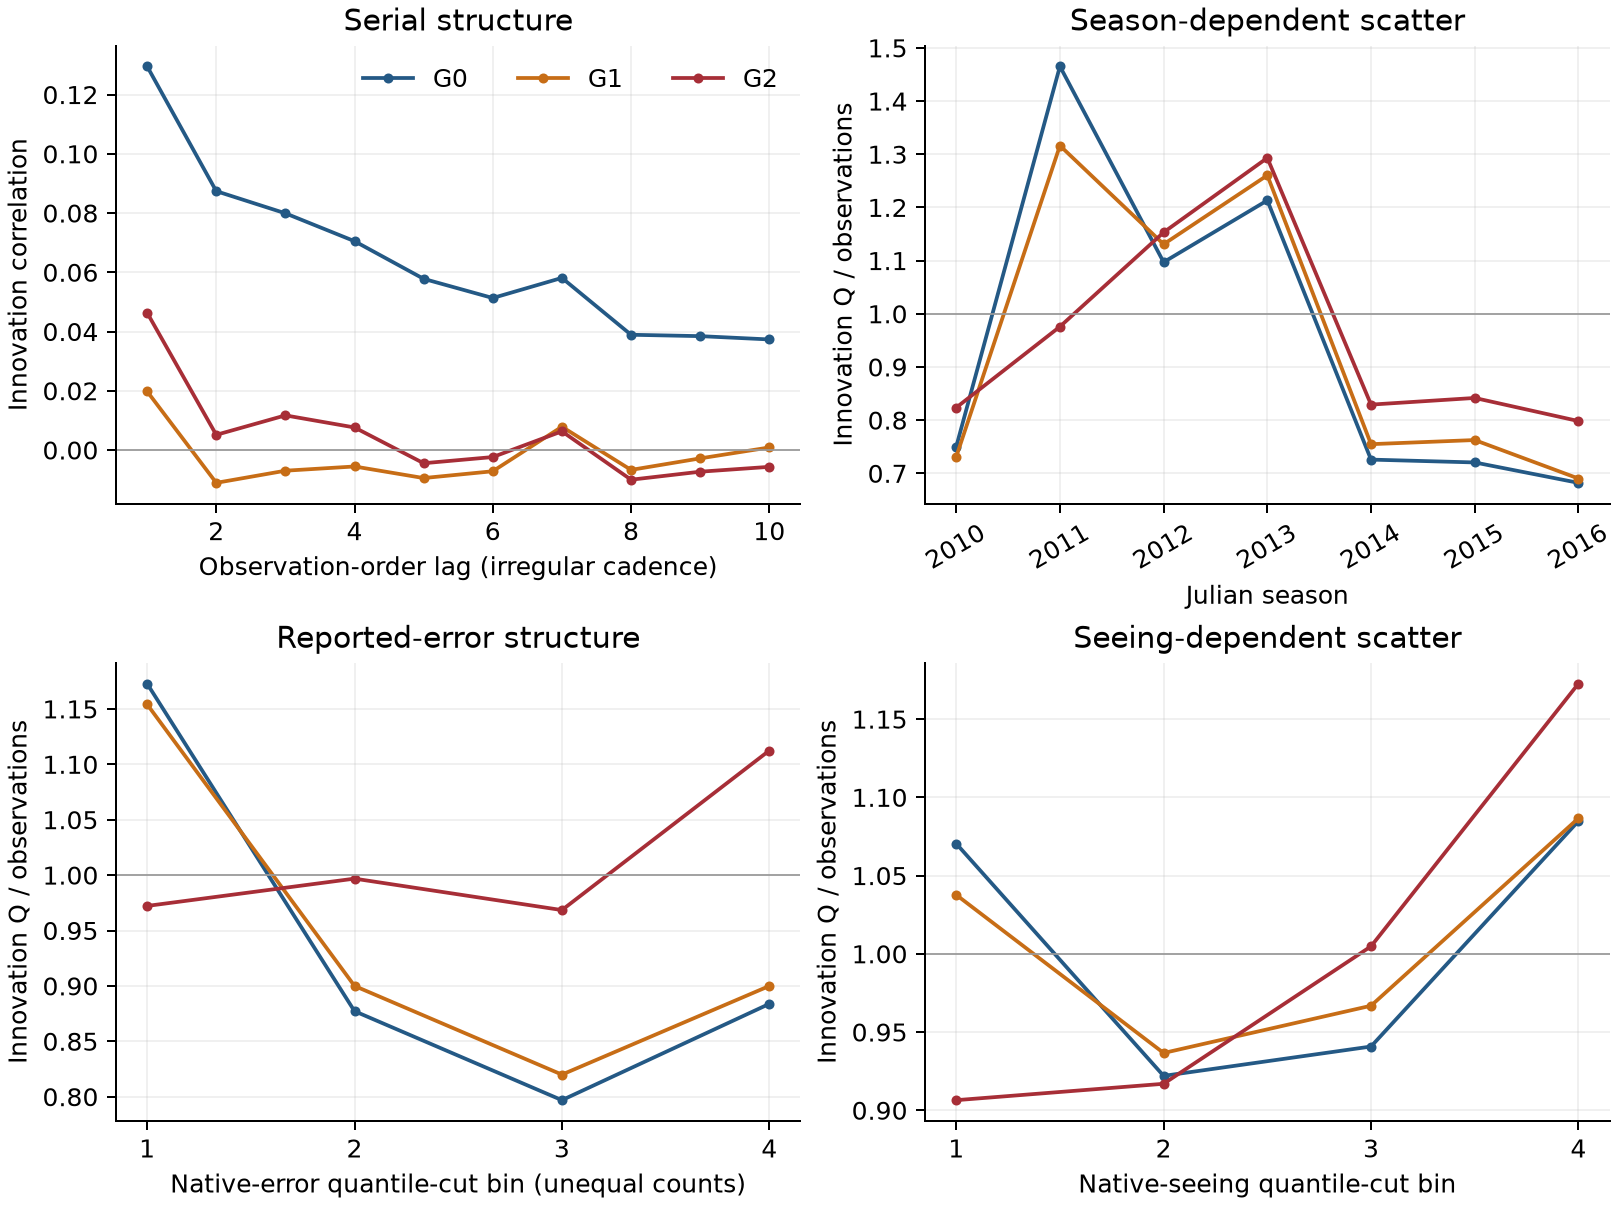
\includegraphics[width=\linewidth]{../joint_known_system_20261022/joint_noise_diagnostics.png}
\caption{Residual structure for the three frozen joint candidates, after the
declared continuation. Global quadratics conceal season, reported-error and
seeing dependence. The reported-error quantile cuts have tied rounded values
and unequal counts $(5817,2874,1787,2022)$; they are not equal-sized samples.
These diagnostic ratios are not calibrated confidence bands.}
\label{fig:joint-noise-failure}
\end{figure}

G0 retains strong serial dependence. G1 removes most short-lag structure and
passes the approximate Ljung--Box screen, but fails native-error, model-brightness,
seasonal, and event/off-event residual checks. G2 fails brightness, seeing, and
seasonal checks, has Ljung--Box probability $6.77\times10^{-5}$, and reaches the
artificial 100~d OU timescale cap. Its lower objective does not establish an
adequate likelihood or a physical timescale limit. Every global quadratic is
apparently acceptable; the failed structure demonstrates why those scalar values
cannot establish trustworthy physical uncertainty.

The corrected whole-night conditional quadratics are $2647.64$ (G1) and
$2540.41$ (G2) for 2464 held-out rows, with approximate two-sided probabilities
$0.01038$ and $0.2771$. Both clear the declared $0.01$ plug-in screen, G1 narrowly.
Their relative Gaussian predictive deviances are $2523.02$ and $2245.68$.
Prediction success cannot override the failed full-data and training residual
structures or the G2 numerical cap. Independent reevaluation of the three saved
baseline states and two saved prediction scores reproduces every checked
quadratic, determinant, and score exactly without refitting.
The original midnight-boundary diagnostics are also retained: for 2467 held-out
rows, G1 has $Q=2710.21$ and approximate probability $0.000768$, while G2 has
$Q=2596.51$ and probability $0.06846$. These values do not supply a whole-night
validation, because that partition splits actual observing nights.

Both fixed 20-control sets are complete. None of the 40 generated/refitted cases
fails a declared residual-variance bin; 19 of 20 in each family pass the overall
screen, with the remaining case rejected by its angular quadratic. Each generated
control family's pass fraction $19/20$ has an exact 95\% binomial interval $[0.751,0.999]$ for
its local generating-model pass probability, rather than mass-interval coverage.
Each measured
lag-one correlation exceeds all 20 corresponding generated values. G1's measured
held-out quadratic also exceeds all its generated values, despite narrowly
passing the plug-in screen. These comparisons reinforce the limitations of a
single scalar screen, but provide only the coarse $1/21$ Monte Carlo tail
resolution. They are local generating-mode checks, rather than global search
or confidence-coverage certification. Ten G2 generating-mass profiles encounter
the numerical timescale cap and remain interval-ineligible.

The completed serial mass grids retain 31 points per OU candidate, without
cross-mass warm starts. G1 has 24 locally eligible and seven cap-limited rows;
crossing refinement gives conditional support $5.989$--$8.399\,M_\odot$ at
$\Delta D=1$ and $5.021$--$9.910\,M_\odot$ at $\Delta D=3.841459$.
These are diagnostic likelihood supports under an inadequate noise hypothesis,
not accepted confidence intervals. Every G2 grid row is cap-limited, and its
32-point refinement gives no eligible crossings or conditional support interval.
An auxiliary parallel scheduling check preserves
the serial results as authoritative: all compared admission states agree, but
some optimizer values differ by up to $0.0133$ in deviance across thread
environments. Three separately repeated points with the same one-thread setting
are identical. No cross-platform numerical identity or profile coverage is
inferred from those checks.

The conditional angular scales range from $4.77$ to $5.18$~mas, whereas the
conditional parallaxes range from $0.0324$ to $0.0971$ and the timescales from
$282.4$ to $340.5$~d. The narrower variation in angular scale is a description of
these fitted models, rather than a validated systematic error bound. In
particular, their mass ratio is not stable across the fixed noise hypotheses.
The software recovers conditional trajectories and angular signals, but this
campaign does not identify a reliably calibrated mass or mass interval.

The protocol therefore stops mass acceptance for every fixed candidate. Diagnostic
profiles and generated controls remain auditable; no additional covariance family
is introduced to make an expected mass appear. Sensitivity calculations cannot
convert an already inadequate baseline into accepted physical inference.
The additional version~2 timing/frame/blend sensitivities are not executed,
because baseline adequacy is their declared entry gate; no robustness to those
systematics is claimed. Earlier version~1 diagnostic sensitivities remain
separately preserved. The
known-system analysis consequently provides no positive demonstration that this
engine can reliably classify unknown black holes. It does demonstrate native-data
ingestion, physical forward prediction, explicit failure detection, and replay.

For a previously unknown object, mass support above a declared compact-object
threshold would still require independent darkness/lens-flux and single-lens
compatibility evidence before a black-hole interpretation. Published darkness
arguments for OB110462 \cite{LamLu2023} are separately attributed; this engine
does not manufacture a new lens-flux limit or assume an absolute distance.
The benchmark does not retrospectively turn the pilot's two archival follow-up
light curves into mass measurements or new black-hole discoveries.

Useful next calibration evidence includes documented
OGLE clock and per-exposure variance components, matched-star and seeing/detector
diagnostics, and exposure-level HST astrometric covariances, reference transforms,
bias corrections, and epoch weights. Absolute frame calibration is separately
required before distance or absolute motion. A new unknown-system interpretation
also needs measured angular-parallax information and independent lens/source
flux constraints. A present-day image cannot manufacture the missing angular
trajectory around a historical photometric peak. These are observational and
calibration requirements, rather than permission to iterate the model until a
black-hole claim passes.

Rejecting these covariance hypotheses does not prove that every estimator using
the observations must fail. Correct-mean estimating equations with cluster/block
robust inference are a separate possible route \cite{LiangZeger1986,CameronMiller2015}.
They still need justified mean/exogeneity and between-block dependence assumptions,
and finite-sample validation for the sparse, unevenly informative HST visits.
Robust uncertainty does not correct a biased mean or shared frame calibration.
No such alternative mass estimator is fitted or validated here, and no reliable
mass support is inferred from the saved G0 point alone.

